%==============================================================================
% Sjabloon poster bachproef
%==============================================================================
% Gebaseerd op document class `a0poster' door Gerlinde Kettl en Matthias Weiser
% Aangepast voor gebruik aan HOGENT door Jens Buysse en Bert Van Vreckem

\documentclass[english,a0,portrait]{hogent-poster}

% Info over de opleiding
\course{Thesis}
\studyprogramme{Applied Information Technology}
\academicyear{2024-2025}
\institution{University of Applied Sciences and Arts Ghent, Valentin Vaerwyckweg 1, 9000 Ghent, Belgium}

% Info over de bachelorproef
\title{AI judge for recognition of jump rope skills in videos.}
% \subtitle{Ondertitel (eventueel)}
\author{Mike De Decker}
\email{mike.dedecker@student.hogent.be}
\supervisor{Ms. L. De Mol \& Mr. T. Parmentier}
\cosupervisor{Mr. D. Plummer (Case Western Reserve University / NextJump)}

% Indien ingevuld, wordt deze informatie toegevoegd aan het einde van de
% abstract. Zet in commentaar als je dit niet wilt.
\specialisation{AI- \& Data Engnineer}
\keywords{Computer vision, Machine Learning, Neural networks, Human Activity Recognition, video classification, YOLO, YOLOv11, MViT, Multiscale Vision Transformer, Swin Transformer, Jump Rope, Rope Skipping, judging, sport}
\projectrepo{https://github.com/mikeddecker/judge}

\begin{document}

\maketitle

\begin{abstract}
Judging the difficulty of jump rope freestyles at high competitive levels, is prone to human errors. It is hard to calculate skill levels, watching multiple athletes at the same time, seeing all actions, skill modifiers or rope manipulations.
Even though a routine consists of forty to sixty skills, wrongly assigning a single level may impact the ranking, deciding national or international selections. In order to correctly assign levels, difficulty judges, at higher level competitions, are allowed to review the routine at slower speeds in order to increase the accuracy of assigned scores.
This is why this research looked for a way to recognize skills in a video. The scope has been limited to recognizing double dutch single freestyles. The solution provided in this research includes a sequential execution of three steps. The first step involves localizing the athletes in order to crop them out of the video. This cropped video can be used in the second step, namely segmenting the video into individual skill sections. Finally, each individual skill section can then be fed into the recognition model, predicting all aspects of the skills performed by the athletes. Training on a skewed limited dataset of less than an hour, containing about 2500 skills, show that more occurring skills reach an accuracy between 80-99\%, while the lesser occurring skills reach a limited accuracy or even none at all. Mapping the skill predictions to scores, averages to minus 20.94\% point difference, compared to the score assigned by judges. Populating the (train and test) dataset with more examples, should greatly increase the accuracy. Not only is this interesting for jump rope, but for other sports or movement analysis in general.

\end{abstract}

\begin{multicols}{2} % This is how many columns your poster will be broken into, a portrait poster is generally split into 2 columns

\section{Introduction}

Jump rope is an evolving sport.
Year after year, an increasing amount of high-level competitors are pushing the limits of jump rope.
This results in new skills, new combinations, better physiques, better rope material, and faster movements. For the judges to keep up with the jumpers and to correctly assess scores to a routine, Double Dutch freestyles, one of the jump rope disciplines, are reviewed at half speed in International competitions or even at nationals in Belgium.
Head judges around the world question the best way to judge athletes correctly so as to give an accurate and objective ranking in competitions.

Thus, this research explored the possibility to recognize skills in double dutch single freestyles.
The proposed solution in this research includes a sequential execution of three steps, namely localizing the athletes, segmenting the video and recognizing the action.
As acquired recordings of videos lose a lot of information on surroundings, it is advised to zoom in on the athletes by cropping them out. These cropped videos can than be used in the segmentation step, which splits the video in various individual skill sections. This way, analysis on full videos can be performed. Thirdly, by labeling the different aspects present in the section, a recognition model can be trained, to predict skills in segmented sections.

Finally, predicted skills can be mapped to their corresponding levels and scores, allowing for judges to review scores on competitions. Not only is this interesting for jump rope, but for other sports like figure skating, synchronized swimming, gymnastics or movement analysis in general.

\section{Jumper Localization}

\href{https://github.com/ultralytics/ultralytics}{Ultralytics} provides an easy-to-use pre-trained implementation of the YOLOv11 model for predicting people and objects in images which can be fine-tuned for specific use cases. Fine-tuning was needed as spectators, also humans, were also included in the predictions.

\begin{center}
  \captionsetup{type=figure}
  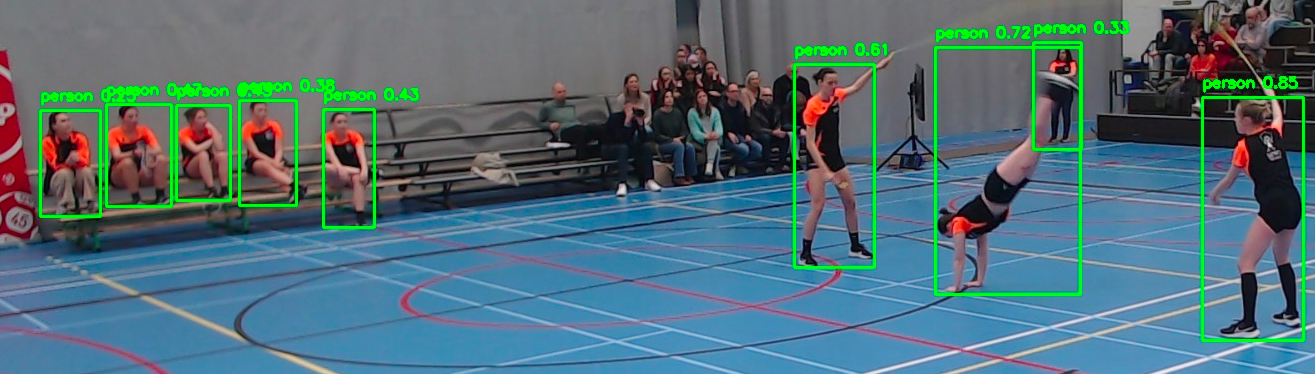
\includegraphics[width=1.0\linewidth]{yolo-raw}
  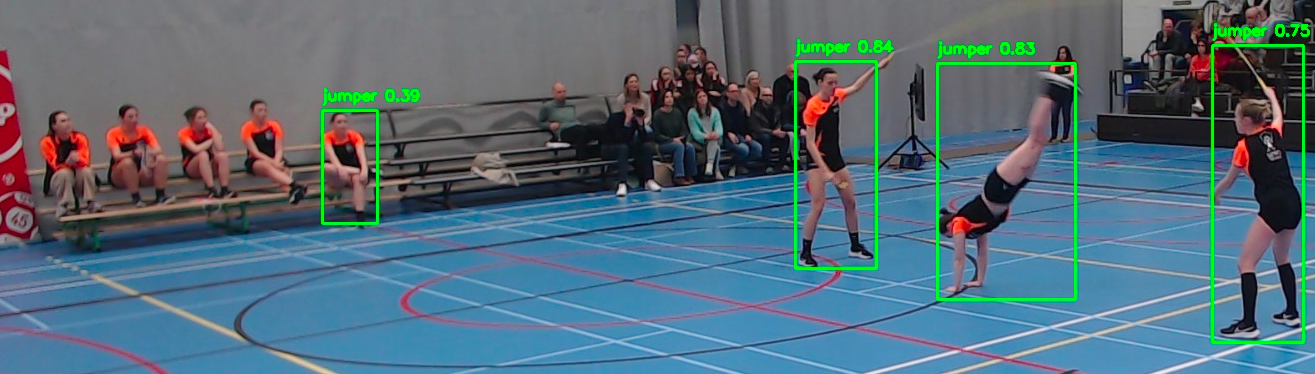
\includegraphics[width=1.0\linewidth]{yolo-finetuned}
  \captionof{figure}{Raw YOLOv11 nano predictions compared to a prediction using fine tuned parameters. The prediction on this video still includes a spectator.}
\end{center}

\begin{center}
  \captionsetup{type=figure}
  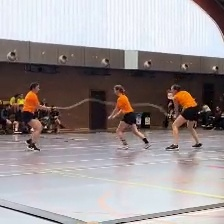
\includegraphics[width=0.32\linewidth]{1315_2935}
  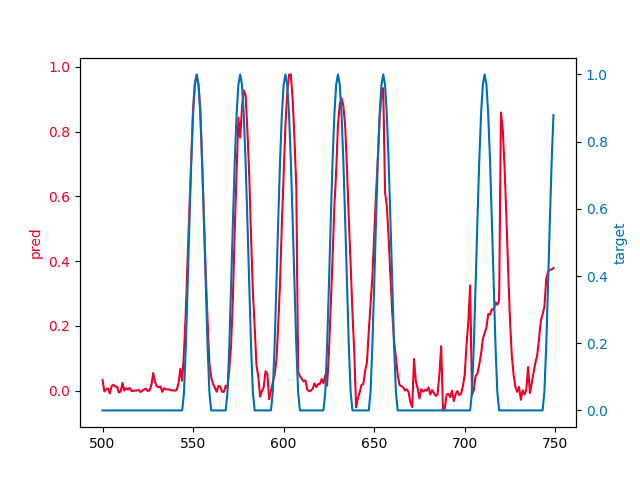
\includegraphics[width=0.45\linewidth]{ai-judge-segment-plot}
  \captionof{figure}{Image on the left: Crop example on a video. (224x224 pixels) \\
  Plot on the right compares the predicted split values points, compared to the label.}
\end{center}

\section{Action segmentation}

Using the cropped videos, actions can be isolated from the video. \href{https://pytorch.org/vision/main/models/video_mvit.html}{PyTorch} has a pre-trained implementation of the \href{10.48550/ARXIV.2104.11227}{Multiscale Vision Transformer (MViT)}.
The pre-trained weights require an input of (1, 3, 16, 224, 224) or (batch size, channels, timesteps, height, width). Thus, a video is split into sequential sections of 16 frames, with a splitvalue between 0 and 1 for each frame. It then predicts 1 output value for each frame. This is illustrated in the segment prediction plot.

\section{Skill recognition}

After segmenting the video, each skills section can be predicted using the \href{10.48550/ARXIV.2104.11227}{Multiscale Vision Transformer} or the \href{https://doi.org/10.48550/arXiv.2103.14030}{Swin Transformer}. However, skills have varying length, which requires frames to be duplicated or skipped in order to create equally sized inputs of (1, 3, 16, 224, 224). Now, for each of the 13 jump rope labels, a prediction can be made. This includes the skill, the type of turning, the number of rotations, first turner, second turner etc. Training on a skewed and limited dataset of about one hour, correctly predicts the most frequent skills between 80-99\%, while the lesser occurring skills reach a limited accuracy or none at all.

\href{https://1drv.ms/v/c/6fa18b11a53f88a6/EWeE_YUHgkVJrhSFT4LIC3UB1WxjQLyZky4oNIUlqaqbQA?e=DBke8i}{Click} or use the link in the Readme of the repo for a video example.

After predicting the skills in a video, levels and scores can be assigned to the routine, which currently differ on average by minus 20.94\%.

\section{Conclusions}

On competitions which use the AI assistant, the actual setting can be adapted in order to have no or less spectators influencing the localization predictions. This then increases further predictions, relying on the localization. Seeing high accuracies on frequent skills, or even starting accuracy on low to mid frequent skills, indicate the possibility of AI recognizable skills. However, a 20\% gap with the scores assigned by judges is to large to consider usable on competitions.

\section{Future research}

This research can be enhanced by other experiments using more models, better metrics for action segmentation, more skill labels of the less occurring skills and skill aspects. Additionally, a benchmark can be created by comparing the score assigned by judges with the ground truth and the AI-models, deciding possible usage at competitions.

To conclude, this research showed the possibilities of the proposed three step architecture for recognizing skills in a full routine on a limited dataset. While results aren't perfect, great effort has been put in the proof of concept, enabling future research, additional labels and additional model experiments.
\end{multicols}
\end{document}